%% myFigures.tex
% A common file to store all figure definitions
%
% In preparing your thesis, one of the first things you should do is
% organize your figures.  Then, one of the last things you'll do is
% reorder your figures so they display where you want them to in the
% text.  Organizing figure definitions in a common files helps:
%
%   1. Write new figures using earlier examples.
%
%   2.  Isolate code and minimize the risk of introducing bugs in the
%   final editing process.  Trust me, moving around just one line of
%   code is easier.
%
%   3.  Reuse figures in other papers.  <=== the best reason!
%
% Note command names can not include numbers and special characters.
%
% To make the file more searchable, use naming conventions that map
% the graphics filename labSetup.jpg to the command name \figlabSetup to the
% figure label fig:labSetup.
% 

%\graphicspath{/5_figures/}

\newcommand{\figCiaTriad}{\begin{wrapfigure}{r}{0.35\textwidth}
 \vspace{-0.8 in}
 \begin{center}
    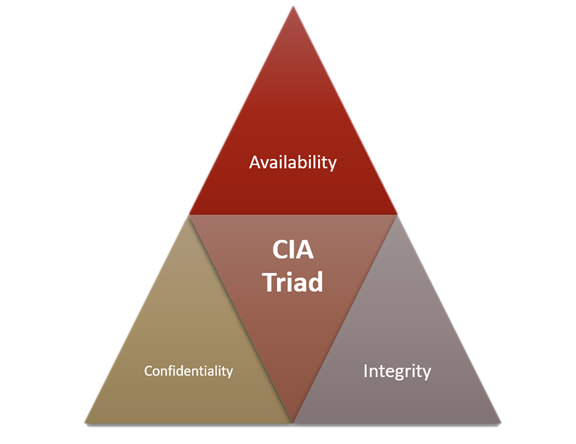
\includegraphics[width=0.35\textwidth]{5_figures/cia_triad.png}
    %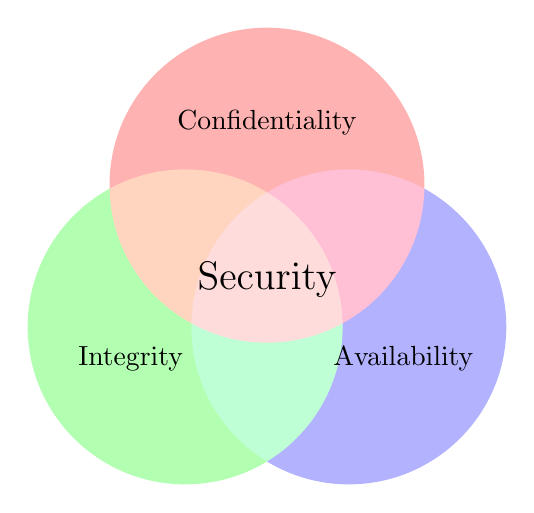
\begin{tikzpicture}
  \begin{scope}[blend group = soft light]
    \fill[red!30!white]   ( 90:1.2) circle (2);
    \fill[green!30!white] (210:1.2) circle (2);
    \fill[blue!30!white]  (330:1.2) circle (2);
  \end{scope}
  \node at ( 90:2)    {Confidentiality};
  \node at ( 210:2)   {Integrity};
  \node at ( 330:2)   {Availability};
  \node [font=\Large] {Security};
\end{tikzpicture}
     \caption{CIA Triad \cite{2018CIATriad}}
     \label{fig:CiaTriad}
 \end{center}
 \vspace{-1.05in}
\end{wrapfigure}
}


\newcommand{\figCiaTree}{\begin{figure}[h]
 \begin{center}
    \tikzset{
  my node style/.style={
    font=\small,
    top color=gray!60,
    bottom color=white!25,
    %fill=green!30,
    rectangle,
    rounded corners,
    minimum size=6mm,
    %draw=black,
    very thick,
    drop shadow,
    align=center,
  }
}
\forestset{
  my tree style/.style={
    for tree={
      parent anchor=south,
      child anchor=north,
      l sep+=5pt,
      my node style,
      edge={draw=black, thick},
      edge path={
        \noexpand\path [draw, \forestoption{edge}] (!u.parent anchor) -- +(0,-7.5pt) -| (.child anchor)\forestoption{edge label};
      },
      if n children=3{
        for children={
          if n=2{calign with current}{}
        }
      }{},
      delay={if content={}{shape=coordinate}{}}
    }
  }
}
\centering
\begin{forest}
  my tree style
  [Security
        [Confidentiality \\ (Privacy)
            %[Content\\Creation]
            %[Content\\Review]
            ]
      [Integrity \\
        [Source\\Authentication]
        [Data\\Verification]
      ]
    [Availability \\
      %[Distributed\\Computing]
      %[Human\\Computing]
    ]
  ]
\end{forest}
     \caption{\gls{adsb} Security Decomposition}
     \label{fig:ciaTree}
 \end{center}
\end{figure}
}


\newcommand{\figAttackClass}{\begin{figure}[h]
 \begin{center}
    \begin{tikzpicture}
  \path[mindmap,concept color=gray,text=white]
    
    node[concept] {\textbf{ADS-B\\Attacks}}
    child[grow=30, concept color=green!50!black] {
      node[concept] {Eaves-\\dropping}
      [clockwise from=90]
      child { node[concept] {Preparatory\\Recon} }
      child { node[concept] {Targeted\\Collection} }
      child { node[concept] {Mass\\Collection} }
    }  
    child[grow=150, concept color=blue] {
      node[concept] {Denial of Service}
      [counterclockwise from=30]
      child { node[concept] {Noise\\Jamming} }
      child { node[concept] {Garbling} }
      child { node[concept] {Preamble\\Flood} }
      child { node[concept] {Message\\Flood} }
      child { node[concept] {Multiple\\False Targets} }
    }
    child[grow=270, concept color=orange] { 
    	node[concept] {Data\\Manipulation} 
        child [grow=35]{ node[concept] {False Target\\Injection} }
        child [grow=345]{ node[concept] {Spoofing} }
        child [grow=295]{ node[concept] {Target Removal} }
        child [grow=245]{ node[concept] {Target Data Mod} }
        child [grow=195]{ node[concept] {Valid Target\\False Data} }
        child [grow=145]{ node[concept] {Replay} }
        };
\end{tikzpicture}
     \caption{\gls{adsb} Attack Classification}
     \label{fig:attackClass}
 \end{center}
\end{figure}
}








\newcommand{\figtitlePage}{\begin{figure}[tbp]
 \begin{center}
    
\includegraphics[width=2in]{5_figures/afitlogo}
     \caption{Enter student data in titlePage.tex to customize the
     document's first pages.}
     \label{fig:titlePage}
 \end{center}
\end{figure}
}

\newcommand{\figmyFlypage}{\begin{figure}[tbp]
 \begin{center}
    \includegraphics[width=6in]{myFlypage}
     \caption{Here we have compiled the first four page of a thesis.}
     \label{fig:myFlypage}
 \end{center}
\end{figure}
}

\newcommand{\figmyFirstAbstract}{\begin{figure}[tbp]
 \begin{center}
    \includegraphics[width=6in]{myFirstAbstract}
     \caption{Add an abstract to the front matter of your thesis.}
     \label{fig:myFirstAbstract}
 \end{center}
\end{figure}
}

\newcommand{\figmyFigures}{\begin{figure}[tbp]
 \begin{center}
    \includegraphics[width=5in]{myFigures}
     \caption{Consider defining all your figures in one file.}
     \label{fig:myFigures}
 \end{center}
\end{figure}
}


\newcommand{\figmyFirstFigures}{\begin{figure}[tbp]
 \begin{center}
    \includegraphics[width=6in]{myFirstFigures}
     \caption{Add figures in the main matter of your document; fill in
     the document around your graphics.}
     \label{fig:myFirstFigures}
 \end{center}
\end{figure}
}

\newcommand{\figmyFirstBibTeX}{\begin{figure}[tbp]
 \begin{center}
    \includegraphics[width=6in]{myFirstBibTeX}
     \caption{Add your bibliography.}
     \label{fig:myFirstBibTeX}
 \end{center}
\end{figure}
}

\newcommand{\figHierarchy}{\begin{wrapfigure}{r}{3in}
    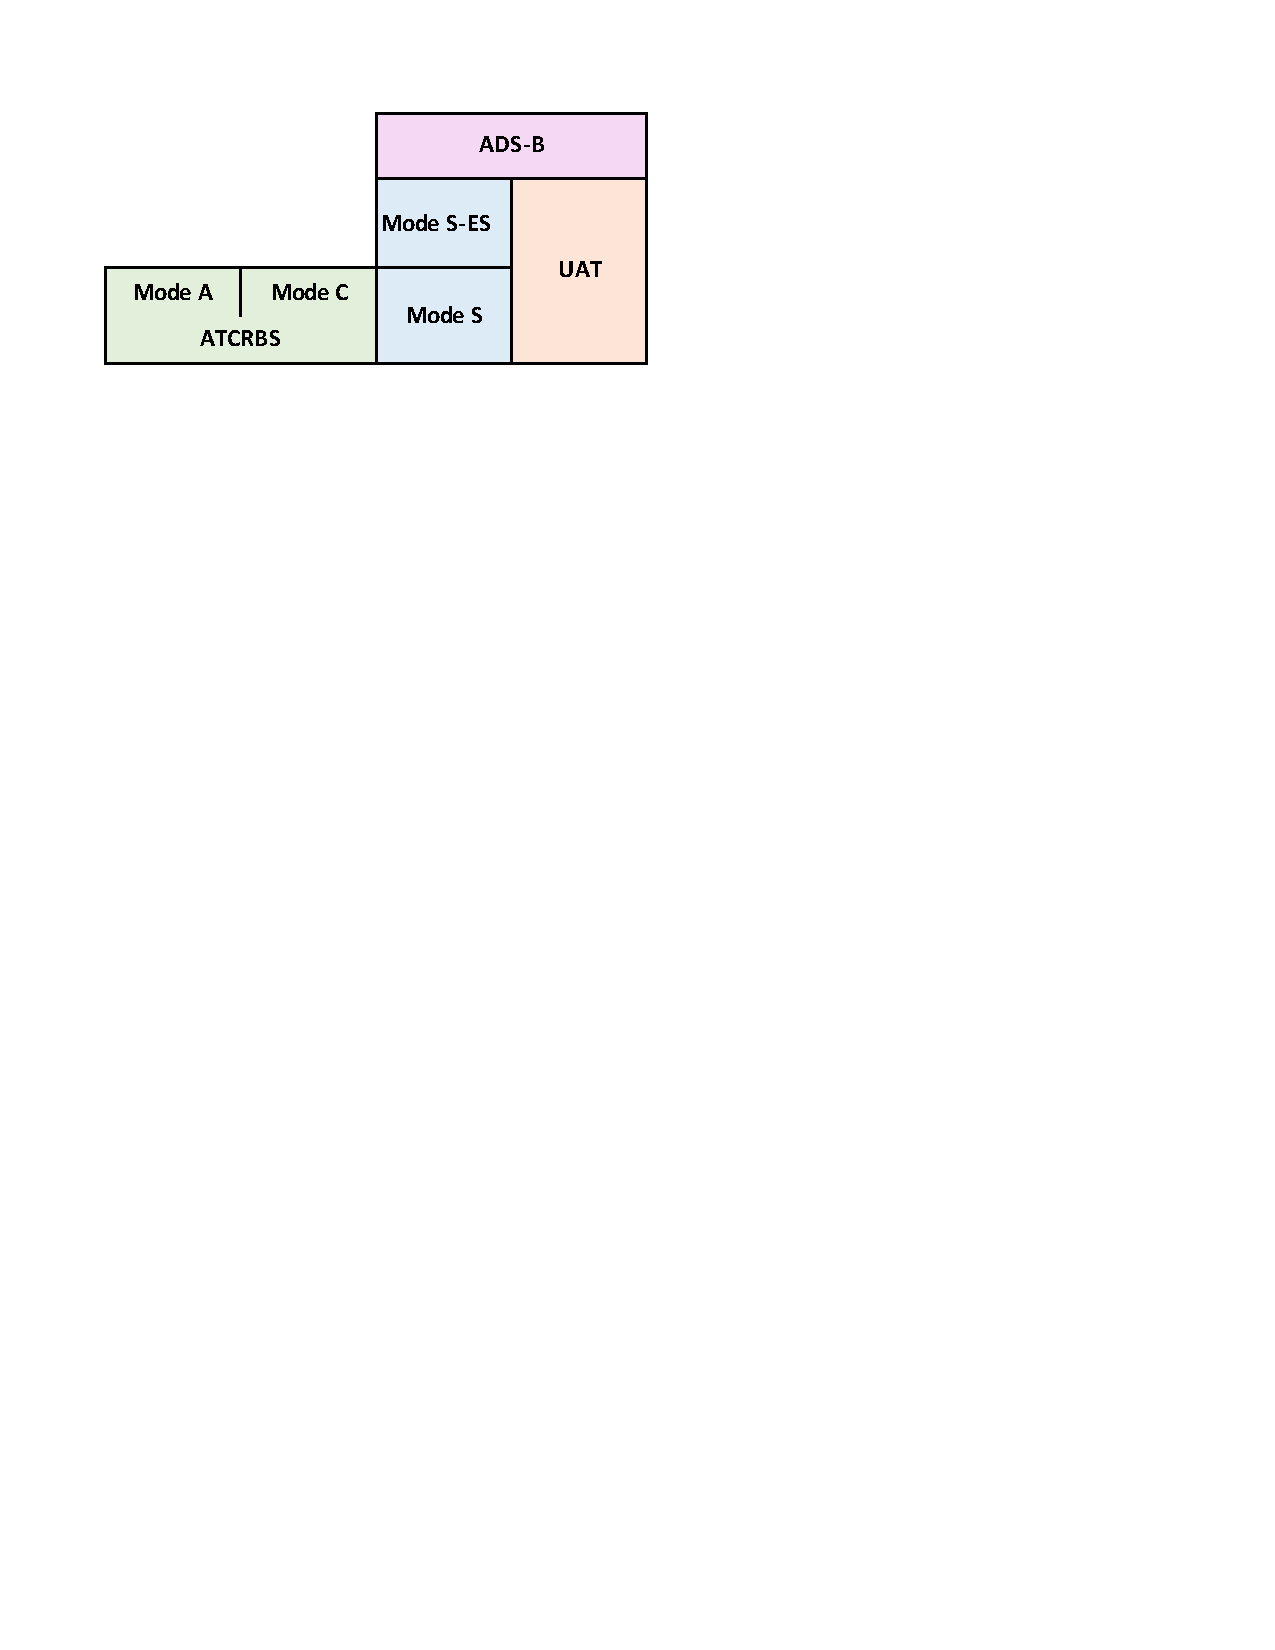
\includegraphics[width=0.5\textwidth]{5_figures/hierarchy}
     \caption{ADS-B Technology}
     \vspace{-0.25in}
     \label{fig:hierarchy}
\end{wrapfigure}
}

\newcommand{\figCoverage}{\begin{wrapfigure}{l}{4in}
    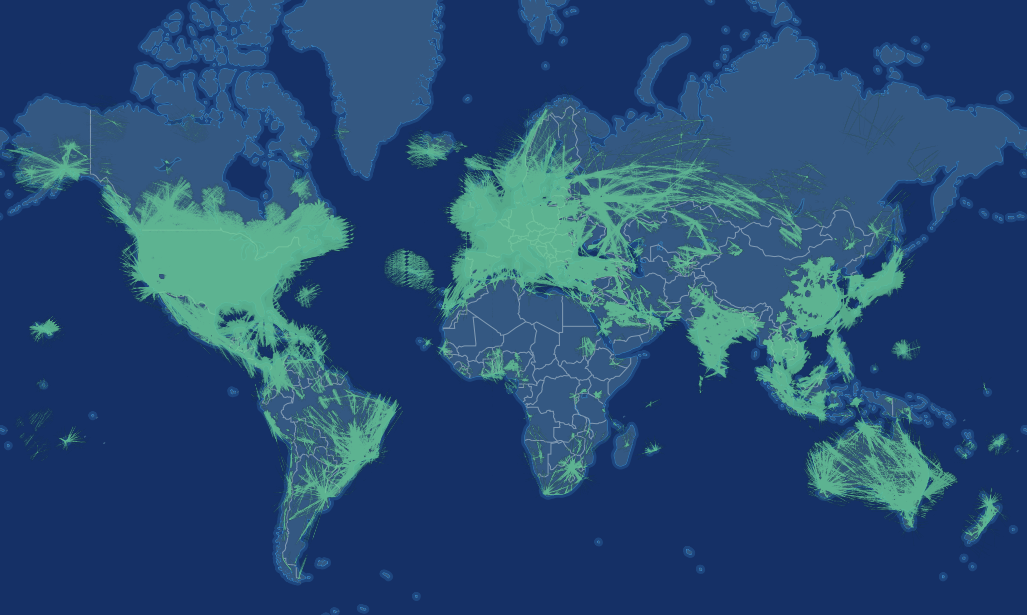
\includegraphics[width=0.65\textwidth]{5_figures/coverage}
     \caption{FlightAware Coverage}
     \vspace{-0.24in}
     \label{fig:coverage}
\end{wrapfigure}
}


